\documentclass[UTF8]{article}
% 中文支持
\usepackage[UTF8]{ctex}	
% pdf调用 封面
\usepackage{pdfpages}
% color宏包
\usepackage{color}  
% 导入图片
\usepackage{caption}
\usepackage{graphicx, subfig}
% 防止图片乱跑
\usepackage{float}
% 支持数学符号
\usepackage{amsmath}
% 支持代码块
\usepackage{listings}
% pdf加入大纲
\usepackage{hyperref}

% 消除报错
\usepackage{lmodern}

% 设置页面的环境,a4纸张大小,左右上下边距信息
\usepackage[a4paper, left=31.8mm, right=31.8mm, top=25.4mm, bottom=25.4mm]{geometry}

% 代码块的基本设置
\lstset{
 columns=fixed,       
 numbers=left,                                        % 在左侧显示行号
 numberstyle=\tiny\color{gray},                       % 设定行号格式
 frame=none,                                          % 不显示背景边框
 backgroundcolor=\color[RGB]{245,245,244},            % 设定背景颜色
 keywordstyle=\color[RGB]{40,40,255},                 % 设定关键字颜色
 numberstyle=\footnotesize\color{darkgray},           
 commentstyle=\it\color[RGB]{0,96,96},                % 设置代码注释的格式
 stringstyle=\rmfamily\slshape\color[RGB]{128,0,0},   % 设置字符串格式
 showstringspaces=false,                              % 不显示字符串中的空格
 language=matlab,                                        % 设置语言
}

\begin{document}

\begin{titlepage}
% 封面信息
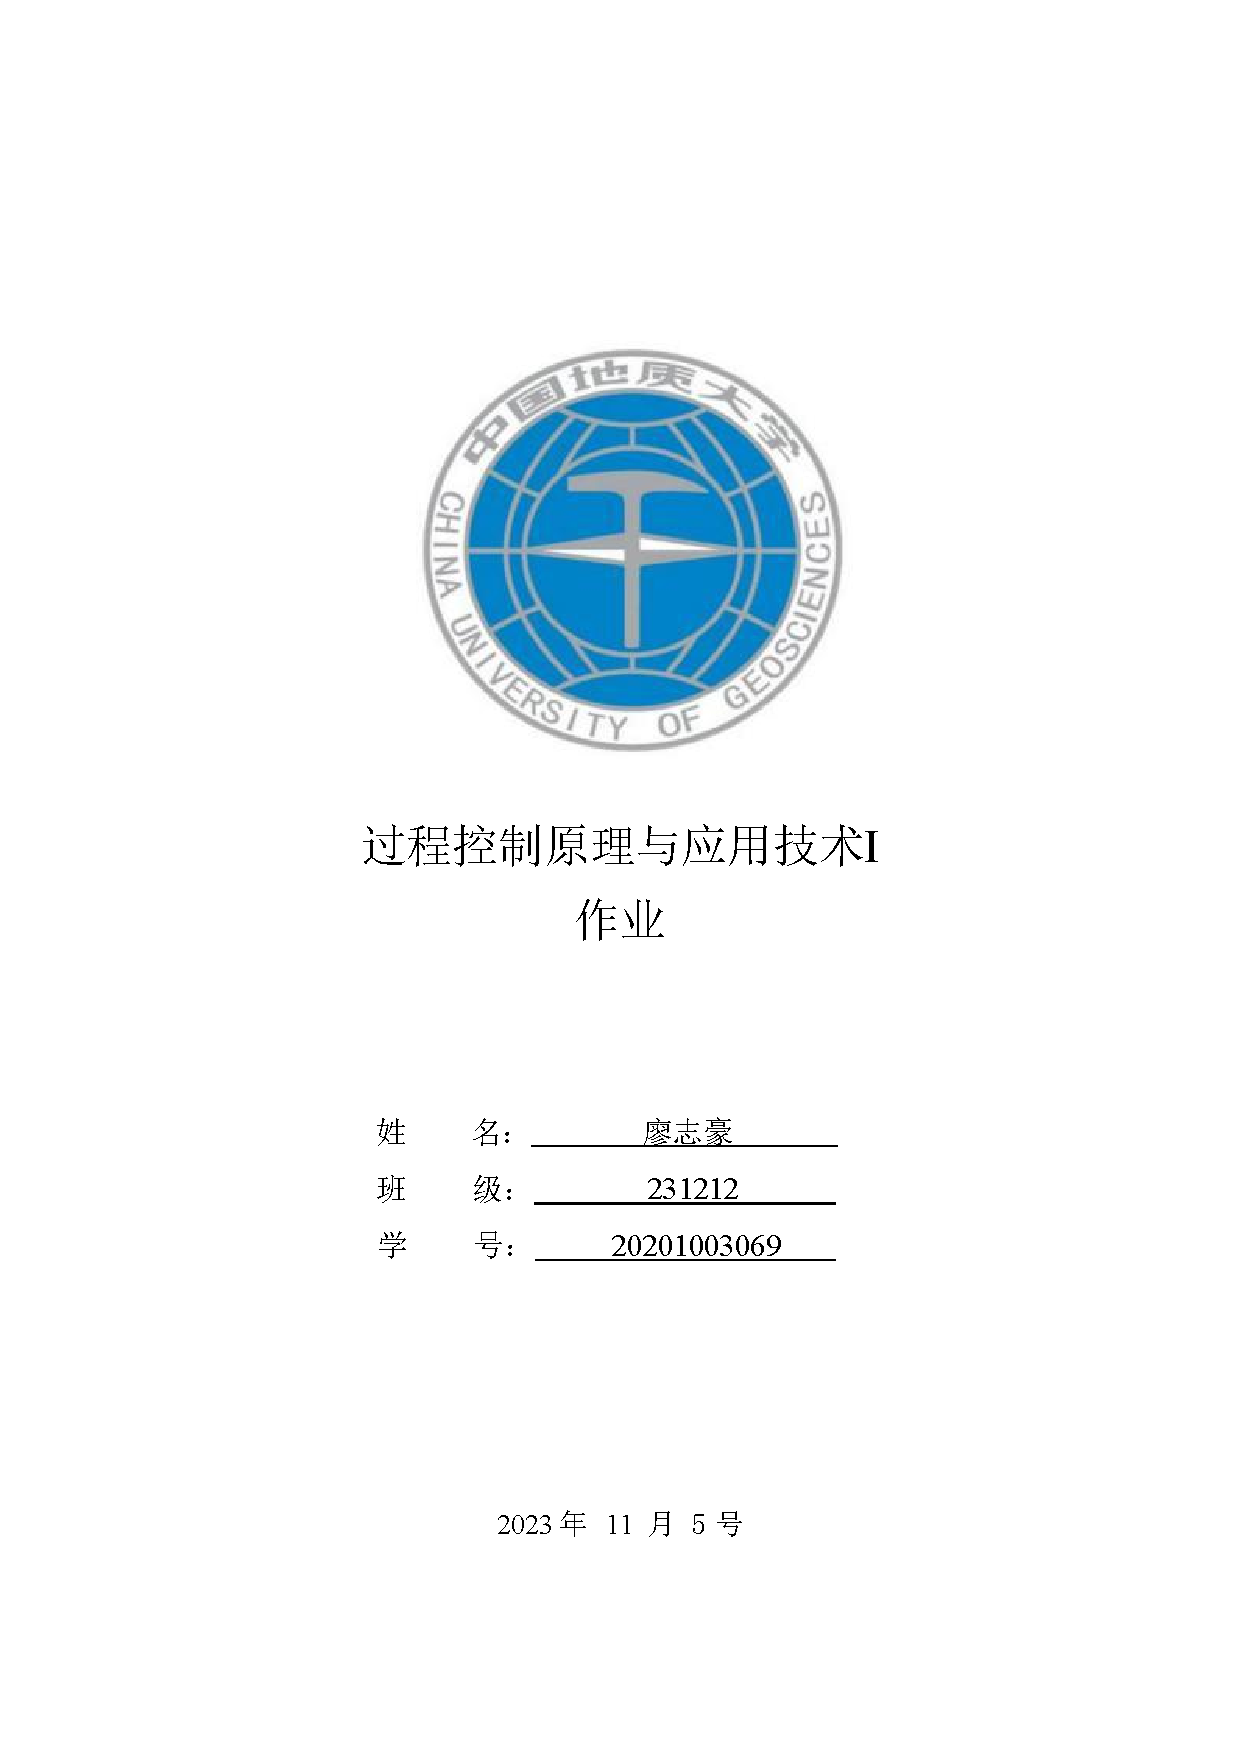
\includepdf[pages={1}]{cover.pdf}
\end{titlepage}

\noindent 题目:对图片进行中值滤波和算数平均值滤波处理。采用matlab编程,编写一个中值滤波函数。
%
\section{思路想法}
图像滤波,即在尽量保留图像细节特征的条件下对目标图像的噪声进行抑制。此处原图加入了椒盐噪声,现利用中值滤波和算数平均值滤波方法分别对图片进行处理,分析处理效果。

%
\section{处理方法}
%%
\subsection{中值滤波}
以一个$3 \times 3$大小的矩阵区域为例,其中有9个像素点,将9个像素点的值进行从小到大排序,得到的中值作为该矩阵区域中心点处像素点的值。对整张图片进行以上操作,即为中值滤波。

%%
\subsection{算数平均值滤波}
以一个$3 \times 3$大小的矩阵区域为例,其中有9个像素点,将9个像素点的值取算数平均值作为该矩阵区域中心点处像素点的值。对整张图片进行以上操作,即为算数平均值滤波。用公式可以表示为:
$$
g(x, y) = \frac{1}{M}\sum_{f \in S} f(x, y)
$$

%
\section{处理过程与处理结果}
%%
\subsection{中值滤波}
\paragraph{处理步骤}
\begin{enumerate}
    \item 读入图像;
    \item 转换为灰度图;
    \item 基于滤波半径分别为$3 \times 3$、$5 \times 5$、$7 \times 7$、$9 \times 9$、$11 \times 11$的中值滤波方法,对原图片进行处理;
    \item 显示处理图片对比结果。
\end{enumerate}

\paragraph{程序}~{}
\\
自行编写的中值滤波函数:
\begin{lstlisting}
function filtered_image = median_filter(input_image, filter_size)
    % 输入参数:
    % input_image - 输入图像(灰度图)
    % filter_size - 滤波器大小,必须是奇数

    % 输出参数:
    % filtered_image - 经过中值滤波处理后的图像

    % 获取输入图像的尺寸
    [rows, cols] = size(input_image);

    % 初始化输出图像
    filtered_image = zeros(rows, cols);

    % 计算滤波器半径
    radius = floor(filter_size / 2);

    % 对每个像素进行中值滤波
    for i = radius + 1:rows - radius
        for j = radius + 1:cols - radius
            % 提取当前像素周围的邻域
            neighborhood = input_image(i - radius:i + radius,...
                j - radius:j + radius);

            % 对邻域进行排序并取中值
            sorted_neighborhood = sort(neighborhood(:));
            median_value = sorted_neighborhood((filter_size * ...
                filter_size + 1) / 2);

            % 将中值赋给输出图像的对应像素
            filtered_image(i, j) = median_value;
        end
    end
    
    %     % 对图像边缘进行额外处理
    %     for x=1:rows
    %         for y = 1:cols
    %             if (x <= radius || y <= radius ||...
    %                   x >= rows-radius || y >= cols-radius)
    %                 filtered_image(x,y)=input_image(x,y);
    %             end
    %         end
    %     end
end
\end{lstlisting}

\noindent 图像处理,主函数部分:
\begin{lstlisting}
%%  中值滤波
clc, clear
% 读入图像
Image = imread('./待处理图片.png');

% 转换为灰度图
Image = rgb2gray(Image);

r3 = median_filter(Image, 3);
r5 = median_filter(Image, 5);
r7 = median_filter(Image, 7);
r9 = median_filter(Image, 9);
r11 = median_filter(Image, 11);

% 展示结果
subplot(2,3,1);imshow(uint8(Image));title('原图');
subplot(2,3,2);imshow(uint8(r3));title('3*3均值滤波结果');
subplot(2,3,3);imshow(uint8(r5));title('5*5均值滤波结果');
subplot(2,3,4);imshow(uint8(r7));title('7*7均值滤波结果');
subplot(2,3,5);imshow(uint8(r9));title('9*9均值滤波结果');
subplot(2,3,6);imshow(uint8(r11));title('11*11均值滤波结果');
\end{lstlisting}

\paragraph{处理结果}~{}
\begin{figure}[H]
    \centering % 居中 
    % 图片文件的相对路径
    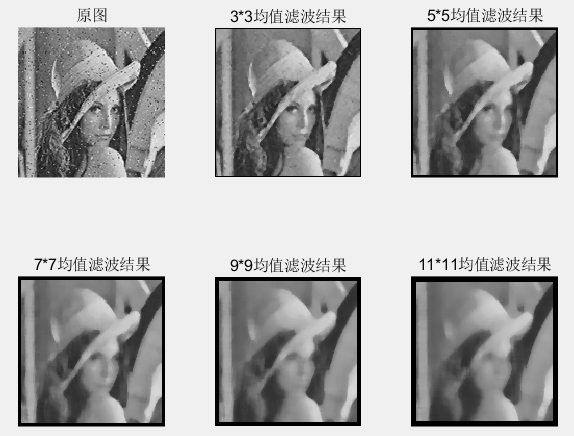
\includegraphics[width=0.8\textwidth]{figure/中值滤波结果.png} 
    \caption{中值滤波不同滤波半径下效果对比图} % caption是图片的标题
    % \label{img} % 此处的label相当于一个图片的专属标志,目的是方便上下文的引用
\end{figure}
由图可以看出,随着中值滤波半径的增大,处理结果越来越模糊。在$3 \times 3$中值滤波处理下,图像相比原图变得更加平滑,噪声基本滤除完毕,滤波效果最为理想。

中值滤波采用非线性方法,在平滑脉冲噪声方面非常有效,可以保护图像尖锐的边缘,对椒盐噪声表现较好。

%%
\subsection{算数平均值滤波}
\paragraph{处理步骤}
\begin{enumerate}
    \item 读入图像;
    \item 创建预定义的滤波算子,设置均值滤波参数分别为$3 \times 3$、$5 \times 5$、$7 \times 7$、$9 \times 9$、$11 \times 11$(为便于处理,一般选择滤波半径为奇数);
    \item 利用均值滤波方法,基于不同滤波参数对图像进行处理;
    \item 显示处理图片对比结果。
\end{enumerate}

\paragraph{程序}~{}

此处的程序实现采用matlab内置的图像滤波方法$imfilter()$,并对比展示了不同均值滤波半径下图片处理的效果:
\begin{lstlisting}
    %% matlab自带均值滤波器
    % 结论:均值滤波半径越大,处理结果越模糊
    clc, clear
    % 读入图像
    Image = imread('./待处理图片.png');
     
    % 设置均值滤波
    H3 = fspecial('average',[3,3]);
    H5 = fspecial('average',[5,5]);
    H7 = fspecial('average',[7,7]);
    H9 = fspecial('average',[9,9]);
    H11 = fspecial('average',[11,11]);
     
    % 利用滤波对图像进行处理
    r3 = imfilter(Image,H3);
    r5 = imfilter(Image,H5);
    r7 = imfilter(Image,H7);
    r9 = imfilter(Image,H9);
    r11 = imfilter(Image,H11);
    
    % 展示结果
    subplot(2,3,1);imshow(Image);title('原图');
    subplot(2,3,2);imshow(r3);title('3*3均值滤波结果');
    subplot(2,3,3);imshow(r5);title('5*5均值滤波结果');
    subplot(2,3,4);imshow(r7);title('7*7均值滤波结果');
    subplot(2,3,5);imshow(r9);title('9*9均值滤波结果');
    subplot(2,3,6);imshow(r11);title('11*11均值滤波结果');
\end{lstlisting}

\paragraph{处理结果}~{}
\begin{figure}[H]
    \centering % 居中 
    % 图片文件的相对路径
    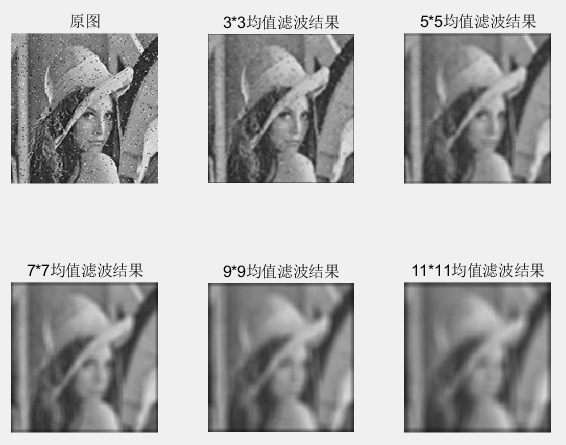
\includegraphics[width=0.8\textwidth]{figure/均值滤波结果.png} 
    \caption{均值滤波不同滤波半径下效果对比图} % caption是图片的标题
    % \label{img} % 此处的label相当于一个图片的专属标志,目的是方便上下文的引用
\end{figure}
由图可以看出,均值滤波半径越大,处理结果越模糊。且在滤波效果最为理想的滤波半径参数设置($3 \times 3$)下,均值滤波的噪声消除效果明显弱于中值滤波。需要注意的一点是,均值滤波本身存在固有的缺陷,不能很好地去除噪声点,不太适合用于此次经椒盐噪声处理后的图像的滤波。
\end{document}